% Preliminary report v0 for the T2->FLAIR course project (IEEE TMI style).
% Build: tectonic -o paper/build paper/main.tex   (sources: paper/, figures: paper/figures/make_figures.py)
% Every number must trace to experiments/<id>/result.json, the preprocessing manifest, paper/data/*.json,
% or a verified literature source (see paper/data/literature.json). Status: results pending.
\documentclass[journal]{IEEEtran}
\usepackage{iftex}
\ifXeTeX\usepackage{fontspec}\setmainfont{texgyretermes}[Extension=.otf,UprightFont=*-regular,BoldFont=*-bold,ItalicFont=*-italic,BoldItalicFont=*-bolditalic]\else\usepackage[T1]{fontenc}\usepackage{newtxtext}\fi
\usepackage{amsmath,amssymb}
\usepackage{array}
\usepackage{graphicx}
\usepackage{booktabs}
\usepackage{multirow}
\usepackage{xcolor}
\usepackage{tikz}
\usetikzlibrary{positioning,arrows.meta,fit,calc}
\usepackage[hidelinks]{hyperref}
\usepackage{cite}

\newcommand{\pend}{\textcolor{gray}{pending}}
\newcommand{\prelim}{$^{\dagger}$}
\newcommand{\Seval}{S_{\mathrm{eval}}}
\newcommand{\Strain}{S_{\mathrm{train}}}

\begin{document}

\title{Lesion-Aware Bridge Flow Matching for T2-to-FLAIR Synthesis: Measuring and Suppressing Lesion-Level Hallucination}

\author{Course project team, ShanghaiTech University (Medical Big Data and AI)%
\thanks{\textbf{Preliminary report v0 (25 Nov 2026).} F1, both segmenters and the evaluation pipeline are implemented and tested; F0 and the lesion-aware losses are not implemented yet; the main F1 training run is queued. Entries marked ``pending'' are not available yet, and numbers marked \prelim{} depend on a
segmenter trained for only 300 steps and will change. No result on the held-out test set has been computed.}}

\maketitle

\begin{abstract}
Synthesizing a missing FLAIR sequence from T2-weighted MRI is attractive because FLAIR is the sequence in which edema and
white-matter lesions are most conspicuous. The same property makes synthesis risky: a generator that erases a lesion or
invents one produces an image that looks plausible but misleads. Recent T2$\to$FLAIR methods, from conditional GANs to
diffusion bridges with wavelet decompositions, are evaluated almost exclusively with image-level PSNR and SSIM, on test sets of 10--20 subjects, often with slice-level or unreported statistics and incompatible preprocessing, so reported numbers cannot be
ranked and lesion fidelity is not measured at all. We propose (i) a lesion-level hallucination protocol that scores
synthetic FLAIR with an independent segmenter, places every method relative to two reference points on the same pipeline (the source T2 itself and real FLAIR), and reports per-subject paired statistics on a 100-subject held-out set of BraTS~2021; (ii) a Brownian-bridge flow
matching model that starts its trajectory at the source T2 slice rather than at noise; and (iii) two lesion-aware training
signals, a lesion-weighted reconstruction loss and a segmentation-consistency loss. We hypothesize that starting from T2
reduces invented lesions at equal image quality, and that the lesion-aware signals reduce missed lesions. This report
describes the method, the protocol, the baselines measured so far, and the planned experiments.
\end{abstract}

\begin{IEEEkeywords}
MRI synthesis, FLAIR, flow matching, diffusion bridge, hallucination, brain tumor, BraTS.
\end{IEEEkeywords}

% ---------------------------------------------------------------------------------------------
\section{Introduction}
\IEEEPARstart{F}{luid}-attenuated inversion recovery (FLAIR) suppresses the signal of cerebrospinal fluid (CSF) while
keeping edema and many lesions hyperintense, which makes it a core sequence for glioma and white-matter disease. When FLAIR
is missing or corrupted, cross-contrast synthesis from an acquired sequence such as T2 can complete the protocol for
downstream tools that expect all four BraTS contrasts~\cite{menze2015brats,baid2021brats}. Compared with T2, the main change
is a largely global, low-frequency contrast inversion of CSF, together with local lesion conspicuity. The global part is
easy to learn; the local part is where synthesis fails silently.

The failure that matters clinically is \emph{lesion-level hallucination}: removing a lesion that is present, or creating
hyperintensities that are not. Hallucination in learned image formation is a recognized risk~\cite{bhadra2021hallucinations},
yet whole-image fidelity metrics are dominated by the large, easy background and CSF regions and barely move when a small
lesion disappears. The same concern is starting to be measured with segmentation-based scores in related
tasks~\cite{kim2026mpflow}.

Published T2$\to$FLAIR results do not measure it. Methods have progressed from conditional
GANs~\cite{isola2017pix2pix,dar2019pgan,dalmaz2022resvit} through conditional diffusion that starts from
noise~\cite{ho2020ddpm,ozbey2023syndiff} to bridges whose trajectory starts at the source image~\cite{li2023bbdm,liu2023i2sb,arslan2025selfrdb},
recently combined with wavelet decompositions~\cite{jiang2025fadm,yang2026wrb}. Their evaluations share three weaknesses
(Section~\ref{sec:lit}): only image-level PSNR/SSIM/MAE (sometimes FID) are reported; test sets have 10--20 subjects, with statistics computed over slices or not specified; and subject subsets, slice ranges and normalizations differ, so the reported values (19--31~dB in Table~\ref{tab:lit}, with the same method, pix2pix, varying by 3.7~dB between papers) cannot be compared across papers. None reports how often lesions are erased or invented.

This work makes three contributions, of which the first is the main one.
\begin{itemize}
\item A \textbf{lesion-level hallucination protocol}: an independent segmenter $\Seval$ scores synthetic FLAIR against the
ground-truth tumor mask (Dice, HD95, false-positive volume away from the tumor, miss rate, small-lesion recall, false alarms
on tumor-free slices), with two reference points on the same pipeline (the T2 input itself and real FLAIR), per-subject
statistics, and a frozen 100-subject test set.
\item \textbf{Bridge flow matching from T2} (F1): a Brownian-bridge flow matching model whose trajectory starts at the
source T2 slice, compared with the same network started from noise (F0) to test hypothesis H1: starting from the source
reduces invented lesions at equal image quality.
\item \textbf{Lesion-aware training}: a lesion-weighted loss and a segmentation-consistency loss added to F1, testing H2:
lesion-aware signals reduce missed lesions without increasing false positives.
\end{itemize}

% ---------------------------------------------------------------------------------------------
\section{Related Work}
\subsection{Adversarial cross-contrast synthesis}
Conditional GANs with an $\ell_1$ term, pix2pix~\cite{isola2017pix2pix} and pGAN~\cite{dar2019pgan}, established paired
multi-contrast MRI synthesis; ResViT~\cite{dalmaz2022resvit} added transformer bottlenecks. Adversarial training gives
sharp images but is known to invent texture where the source is ambiguous, which is precisely the lesion failure mode.

\subsection{Conditional diffusion from noise}
Denoising diffusion models~\cite{ho2020ddpm,dhariwal2021adm} conditioned on the source contrast start from Gaussian noise and
need many steps; SynDiff~\cite{ozbey2023syndiff} combined adversarial diffusion with cycle consistency for MRI translation.
Because the starting point is independent of the source, all source information must enter through conditioning.

\subsection{Diffusion bridges and frequency-aware bridges}
Bridges place the source image at one end of the stochastic trajectory: BBDM~\cite{li2023bbdm} uses a Brownian bridge,
I$^2$SB~\cite{liu2023i2sb} a Schr\"odinger bridge, and SelfRDB~\cite{arslan2025selfrdb} adds a self-consistent recursive
estimate of the target with few sampling steps; SelfRDB is a recent bridge method with released code and weights. FADM~\cite{jiang2025fadm}
runs an I$^2$SB-style bridge on Haar sub-bands with a high-frequency supervision module, and WRB~\cite{yang2026wrb} maps
low-frequency wavelet coefficients deterministically and samples only low-rank high-frequency residuals with a bridge.
Neither releases code. All of them evaluate with image-level metrics only.

\subsection{Flow matching and stochastic interpolants}
Flow matching~\cite{lipman2023flowmatching}, rectified flow~\cite{liu2023rectifiedflow} and stochastic
interpolants~\cite{albergo2023interpolants,albergo2025unifying} learn transport between arbitrary endpoint distributions with a
simulation-free regression loss; bridge matching~\cite{shi2023dsbm} specializes this to paired or coupled endpoints. A recent
MRI benchmark found that flow matching can overfit on small data where pix2pix remains competitive~\cite{moschetto2025benchmark},
and tumor-aware constraints have been added to flow matching for contrast-enhanced synthesis~\cite{chang2025controllable}. We use a
bridge interpolant between paired T2 and FLAIR slices with a small stochastic term, so the start point is the source image.

\subsection{Measuring hallucination}
Bhadra et al.~\cite{bhadra2021hallucinations} formalized hallucinations in tomographic reconstruction. In MRI, downstream
segmentation of the synthesized image is the most direct proxy for lesion fidelity; MPFlow~\cite{kim2026mpflow} reports tumor
hallucination through the Dice of a segmenter trained on real FLAIR. We adopt this idea for synthesis and make it a full
protocol: a segmenter that is independent of training, an identity reference and a real-image reference, and
lesion-level error types rather than a single Dice.

% ---------------------------------------------------------------------------------------------
\section{Method}
\label{sec:method}

\begin{figure*}[t]
\centering
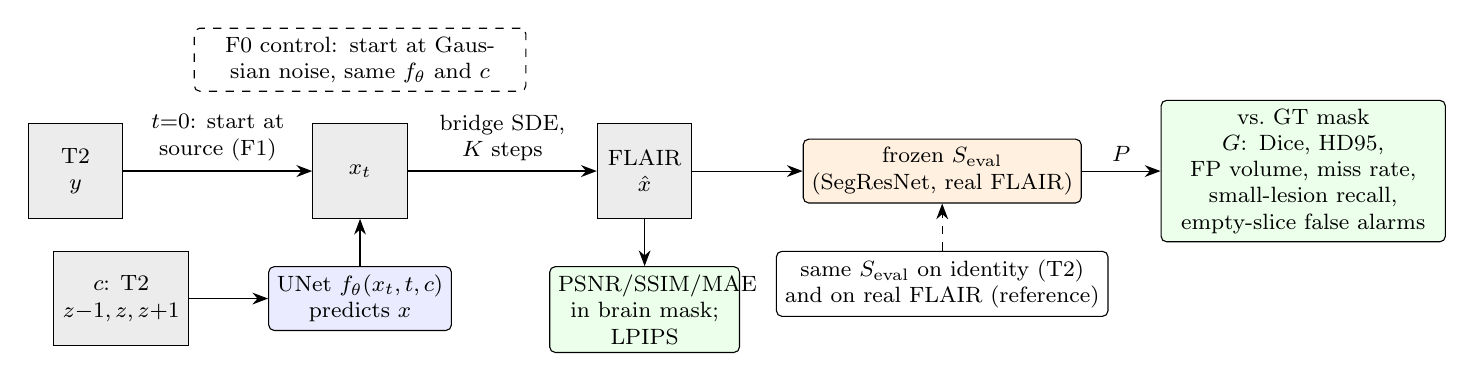
\begin{tikzpicture}[
  font=\footnotesize, >={Stealth[length=2mm]},
  box/.style={draw, rounded corners=2pt, align=center, minimum height=8mm, inner sep=3pt},
  img/.style={draw, fill=gray!15, minimum width=12mm, minimum height=12mm, align=center},
  net/.style={box, fill=blue!8},
  seg/.style={box, fill=orange!12},
  met/.style={box, fill=green!8}]
% generation
\node[img] (t2) {T2\\ $y$};
\node[img, right=24mm of t2] (xt) {$x_t$};
\node[img, right=24mm of xt] (fl) {FLAIR\\ $\hat x$};
\draw[->, thick] (t2) -- node[above, align=center]{$t{=}0$: start at\\ source (F1)} (xt);
\draw[->, thick] (xt) -- node[above, align=center]{bridge SDE,\\ $K$ steps} (fl);
\node[net, below=6mm of xt] (unet) {UNet $f_\theta(x_t, t, c)$\\ predicts $x$};
\node[img, left=10mm of unet, minimum width=10mm] (cond) {$c$: T2\\ $z{-}1,z,z{+}1$};
\draw[->] (cond) -- (unet);
\draw[->] (unet) -- (xt);
\node[box, above=4mm of xt, dashed, text width=40mm] (f0) {F0 control: start at Gaussian noise, same $f_\theta$ and $c$};
% evaluation
\node[seg, right=14mm of fl] (seval) {frozen $\Seval$\\ (SegResNet, real FLAIR)};
\draw[->] (fl) -- (seval);
\node[met, right=10mm of seval, text width=34mm] (m) {vs.\ GT mask $G$: Dice, HD95,\\ FP volume, miss rate,\\ small-lesion recall,\\ empty-slice false alarms};
\draw[->] (seval) -- node[above]{$P$} (m);
\node[box, below=6mm of seval, text width=40mm] (refs) {same $\Seval$ on identity (T2) and on real FLAIR (reference)};
\draw[->, dashed] (refs) -- (seval);
\node[met, below=6mm of fl, text width=22mm] (img) {PSNR/SSIM/MAE in brain mask; LPIPS};
\draw[->] (fl) -- (img);
\end{tikzpicture}
\caption{Overview. \emph{Left}: F1 transports the source T2 slice $y$ to FLAIR along a Brownian bridge; a UNet conditioned
on three adjacent T2 slices $c$ predicts the clean target $x$ from $x_t$. F0 uses the same network but starts from noise.
\emph{Right}: lesion-level evaluation. A frozen segmenter $\Seval$, trained only on real training FLAIR and never used in
training the generator, segments the synthetic volume; its errors against the ground-truth mask are compared with those of the same segmenter on the
identity input and on real FLAIR.}
\label{fig:overview}
\end{figure*}

\subsection{Problem and data contract}
Let $y\in[-1,1]^{H\times W}$ be an axial T2 slice and $x$ the co-registered FLAIR slice of the same subject. Each volume
and contrast is normalized separately: intensities inside the brain (voxels $>0$) are clipped at their 99.5th percentile
and mapped linearly to $[-1,1]$, with background fixed at $-1$; no per-slice normalization is applied. We keep axial
slices whose brain fraction exceeds 10\% and center-crop to $192\times192$. The network sees a 2.5D condition
$c=(y_{z-1},y_z,y_{z+1})$ (edge slices repeated); the bridge starts at $y=y_z$. The whole-tumor mask $M$ (BraTS label
$>0$) is used only for the lesion-aware losses and for evaluation, never at inference.

\subsection{Bridge flow matching from T2 (F1)}
For $t\in[0,1]$ we use the Brownian-bridge interpolant between source and target,
\begin{equation}
x_t = (1-t)\,y + t\,x + \sigma\sqrt{t(1-t)}\,\varepsilon,\qquad \varepsilon\sim\mathcal N(0,I),
\label{eq:interp}
\end{equation}
so $x_0=y$ and $x_1=x$. A network $f_\theta$ predicts the endpoint directly and is trained with
\begin{equation}
\mathcal L_{\mathrm{FM}} = \mathbb E_{t\sim\mathcal U(0,1),\,\varepsilon}\big\|f_\theta(x_t,t,c)-x\big\|_2^2 .
\label{eq:loss}
\end{equation}
Sampling uses $K$ uniform steps $t_k=k/K$ starting from $x_{t_0}=y$. At each step we predict $\hat x=\mathrm{clip}(f_\theta(x_{t_k},t_k,c),-1,1)$
and draw from the bridge posterior between $x_{t_k}$ and $\hat x$:
\begin{equation}
x_{t_{k+1}} = x_{t_k} + \tfrac{\Delta}{1-t_k}\,(\hat x - x_{t_k}) + \sigma\sqrt{\tfrac{\Delta\,(1-t_{k+1})}{1-t_k}}\;z,
\label{eq:sampler}
\end{equation}
with $\Delta=t_{k+1}-t_k$ and $z\sim\mathcal N(0,I)$; the last step returns $\hat x$. With an oracle $\hat x=x$, the
marginal of~\eqref{eq:sampler} at every $t_k$ equals that of~\eqref{eq:interp}, which we check in a unit test. We use
$\sigma=0.5$ and $K=50$ for evaluation. Because the trajectory starts at the observed T2, large regions that only need a
contrast change (CSF, background) never pass through noise; we hypothesize that this leaves less room for invented structure than starting from noise.

\emph{Relation to bridge diffusion.} With endpoint prediction and the stochastic sampler~\eqref{eq:sampler}, F1 is closely
related to BBDM~\cite{li2023bbdm} and I$^2$SB~\cite{liu2023i2sb}; \eqref{eq:interp} is a stochastic
interpolant~\cite{albergo2023interpolants,albergo2025unifying} with Brownian-bridge noise, and $\sigma\to0$ gives a
straight-line flow between T2 and FLAIR. We call it bridge flow matching because training is a simulation-free regression on
this interpolant, but we do not claim the bridge itself as new: our claim is limited to the controlled comparison with F0
(identical network, data and budget) and its effect on lesion-level errors.

\subsection{Noise-start control (F0)}
F0 keeps the network, condition, loss target and training budget of F1 but replaces the start point $y$ by Gaussian
noise, i.e.\ conditional flow matching in the sense of~\cite{lipman2023flowmatching}. F0 isolates the effect of the start point
(H1); it will be added as a switch in the same code path \emph{(not implemented yet)}.

\subsection{Lesion-aware training (planned ablations)}
\emph{Lesion-weighted loss.} We replace~\eqref{eq:loss} by a per-pixel weighted error with
$W=1+(\alpha-1)\,\mathrm{dilate}(M)$, $\alpha=5$, so errors in and around the tumor cost more.
\emph{Segmentation consistency.} A frozen segmenter $\Strain$, trained on real training FLAIR, segments the predicted
endpoint $\hat x=f_\theta(x_t,t,c)$; a Dice+BCE loss against $M$ is added with weight $\lambda$, only for $t>0.5$ where
$\hat x$ is reliable. $\Strain$ and the evaluation segmenter $\Seval$ differ in architecture and seed. Because both are trained on the same images and labels, this reduces but does not rule out shortcuts that satisfy the evaluator; we will report the agreement of $\Strain$ and $\Seval$ on generated images. Dilation radius and $\lambda$ will be fixed in the ablation cards before running.

\subsection{Lesion-level evaluation}
\label{sec:eval}
$\Seval$ is a 2D SegResNet~\cite{myronenko2018segresnet} (MONAI~\cite{cardoso2022monai}) and $\Strain$ a 2D
U-Net~\cite{ronneberger2015unet} (MONAI BasicUNet); both map one FLAIR slice to a whole-tumor logit, are trained on
\texttt{main\_train} real FLAIR only (soft Dice+BCE, 20k steps), are selected by mean 3D Dice on \texttt{main\_val}, and are
then frozen. For each subject, slice predictions are thresholded at 0.5 and stacked into a 3D mask $P$ and compared with
the ground truth $G$:
\begin{itemize}
\item Dice$(P,G)$ and symmetric HD95;
\item false-positive volume $|P\setminus\mathrm{dilate}(G,5)|$ (invented lesions away from the tumor);
\item miss rate $1-|P\cap G|/|G|$ (erased lesion);
\item small-lesion recall: fraction of GT connected components $<1000$ voxels touched by $P$ (pooled over subjects);
\item empty-slice false-alarm rate: fraction of tumor-free slices with $|P|>20$ pixels (pooled).
\end{itemize}
The same $\Seval$ is applied to the identity input (the T2 slice itself) and to real FLAIR; the latter shows what the evaluator achieves on real images.
Neither is a bound: a generator can produce more false positives than identity, or exceed real FLAIR by exaggerating lesion
contrast. Small-lesion recall counts GT components below 1000 voxels; in glioma most of these are satellites of the main
mass, so it is a secondary, exploratory metric. Image quality is measured with PSNR, SSIM~\cite{wang2004ssim} and MAE inside
the brain mask after mapping $[-1,1]\to[0,1]$, and LPIPS~\cite{zhang2018lpips} (AlexNet) on the full slice.

\emph{Validity of the evaluator.} $\Seval$ is trained on real FLAIR and applied to synthetic images, so part of a Dice gap
can be a domain shift of the evaluator rather than a lesion error. Applied to T2, $\Seval$ is far out of distribution, so
identity Dice measures the segmenter's response to T2 hyperintensities rather than lesion fidelity. Before interpreting
Dice differences between generators we will (i) apply $\Seval$ to real FLAIR degraded by blur and noise matched to each
generator's image error, and (ii) report the per-subject correlation between image error and Dice change.

\subsection{Implementation}
$f_\theta$ is a 2D UNet (diffusers \texttt{UNet2DModel}; base width 64, multipliers $1,2,4,8$, two residual blocks per level,
self-attention at $48^2$ and $24^2$ with 64 channels per head; 63.2M parameters) taking $(x_t,c)$ as four input channels.
Training: AdamW, learning rate $10^{-4}$ with 1k-step warm-up and then constant, batch 64, 50k steps (about 106 epochs of the
30{,}277 training slices), EMA 0.9999, gradient clipping 1.0, bf16, horizontal flips only. The checkpoint is selected by
brain-mask PSNR of EMA samples (10 steps) on a fixed subset of \texttt{main\_val}. A pre-registered extension rule continues
training once to 80k steps if the best validation PSNR at 45k/50k exceeds that at 40k by more than 0.3~dB. On one A100
80GB PCIe this runs at a measured 1.36 it/s (about 10.2 h). Moving from the library default of 8 channels per attention head to 64
gave a $1.31\times$ speed-up without changing the parameter count; the data loader and TF32 were not bottlenecks.

% ---------------------------------------------------------------------------------------------
\section{Experiments}
\subsection{Data and splits}
We use the BraTS 2021 training set~\cite{baid2021brats,menze2015brats,bakas2017advancing} (1251 glioma subjects; co-registered,
skull-stripped, 1~mm, $240\times240\times155$). Splits are by subject. The \emph{main} protocol draws 430 subjects with a
fixed seed into 300 training, 30 validation and 100 test subjects (30{,}277 / 3{,}077 / 10{,}083 kept slices). Center
cropping removes at most 0.29\% of any subject's brain voxels and no tumor voxels. The test set is frozen: it is not used for
model selection, early stopping or hyper-parameters, and is evaluated once at the end. A second \emph{literature} protocol
(25/5/10 subjects, axial slices 27--126, generated with the public split script of D3Bridge~\cite{xie2026d3bridge}) mirrors the setting of~\cite{yang2026wrb} and is used only to show how much the
protocol, rather than the method, moves PSNR.

\subsection{Statistics}
Metrics are computed per subject and summarized as mean $\pm$ s.d.\ over subjects, except small-lesion recall and
empty-slice false alarms, which are pooled ratios and are compared with a subject-level bootstrap. Subjects with an empty
prediction have undefined HD95; their number is reported (a fixed penalty value is an open choice). Each hypothesis gets one
primary endpoint with a non-inferiority margin, fixed in its experiment card before running: for H1, the paired difference
in false-positive volume between F1 and F0, with PSNR non-inferiority (e.g.\ $-0.5$~dB, two one-sided tests); for H2, the
paired difference in miss rate, with false-positive non-inferiority. Primary endpoints are tested with paired Wilcoxon
signed-rank tests over subjects, Holm-corrected across hypotheses, with 95\% bootstrap confidence intervals; all other
metrics are exploratory. The trunk experiment itself is judged on PSNR relative to identity and on $\Seval$ Dice relative to
real FLAIR. Model selection uses \texttt{main\_val} (the generator on an 8-subject subset, the segmenters on all 30
subjects), so \texttt{main\_val} numbers are optimistic, the real-FLAIR reference in particular; \texttt{main\_test} gives
the unbiased estimate. With 30 subjects only large paired effects are detectable; a minimum detectable effect will be
computed from the trunk's per-subject spread.

\subsection{Compared methods}
Identity (output the T2 slice); UNet-$\ell_1$ regression (same UNet, direct prediction); pix2pix~\cite{isola2017pix2pix};
SelfRDB~\cite{arslan2025selfrdb}, retrained on our split with its released code; F0; F1; F1 with each lesion-aware loss.
WRB and FADM have no public code and are discussed through their reported numbers only.

\subsection{Reported results in the literature}
\label{sec:lit}
\begin{table*}[t]
\centering
\caption{Reported BraTS T2$\to$FLAIR results. Values are copied from each paper's table; protocols differ, so rows from different papers are \emph{not} comparable. SSIM in \%. Selected rows; FADM and ResViT SSIM converted from $[0,1]$. $^{\ddagger}$: digits identical (or one digit apart) to a row of the SelfRDB paper's Table~2 obtained under a different protocol, in two cases for a differently named method (WRB ``BBDM'' = SelfRDB ``I$^2$SB''; WRB ``CycleGAN'' mean and SSIM = SelfRDB ``SAGAN'').}
\label{tab:lit}
\footnotesize
\setlength{\tabcolsep}{3pt}
\resizebox{\textwidth}{!}{%
\begin{tabular}{llccl|l}
\toprule
Source & Method & PSNR (dB) & SSIM (\%) & Source table & Protocol of the source \\
\midrule
WRB~\cite{yang2026wrb} & pix2pix$^{\ddagger}$ & 24.85$\pm$1.57 & 83.36$\pm$3.11 & Tab.~1 & BraTS'21, 25/5/10 subj.; slices 27--126; per-slice $[0,1]$; foreground mask; per-slice stats \\
 & CycleGAN$^{\ddagger}$ & 27.08$\pm$3.42 & 87.59$\pm$2.93 &  &  \\
 & BBDM$^{\ddagger}$ & 25.92$\pm$2.00 & 83.51$\pm$4.05 &  &  \\
 & DDPM$^{\ddagger}$ & 26.90$\pm$1.84 & 87.86$\pm$2.85 &  &  \\
 & SelfRDB & 26.84$\pm$1.88 & 90.59$\pm$2.79 &  &  \\
 & WRB & 27.51$\pm$1.00 & 91.33$\pm$2.07 &  &  \\
\midrule
FADM~\cite{jiang2025fadm} & CycleGAN & 19.21$\pm$2.61 & 82.7$\pm$5.7 & Tab.~2 & BraTS'21, 80/10/10; 70 slices/subj.; resized to 256; norm., mask, unit not reported \\
 & pix2pix & 25.91$\pm$3.72 & 83.7$\pm$4.7 &  &  \\
 & SR3 & 27.49$\pm$2.01 & 86.9$\pm$3.7 &  &  \\
 & I$^2$SB & 29.21$\pm$2.44 & 93.7$\pm$2.4 &  &  \\
 & FADM & 30.85$\pm$1.34 & 95.8$\pm$2.5 &  &  \\
\midrule
SelfRDB~\cite{arslan2025selfrdb} & pix2pix & 26.85$\pm$1.57 & 86.36$\pm$3.11 & Tab.~2 & BRATS, 25/10/20; 100 slices/subj.; volume mean-norm.; mask not stated \\
 & SAGAN & 27.08$\pm$1.57 & 87.59$\pm$2.93 &  &  \\
 & DDPM & 26.90$\pm$1.84 & 87.86$\pm$2.85 &  &  \\
 & SynDiff & 27.77$\pm$1.77 & 89.62$\pm$2.87 &  &  \\
 & I$^2$SB & 25.92$\pm$2.00 & 83.51$\pm$4.05 &  &  \\
 & SelfRDB & 27.98$\pm$1.80 & 90.01$\pm$2.70 &  &  \\
\midrule
SynDiff~\cite{ozbey2023syndiff} & cGAN & 27.41$\pm$0.78 & 88.48$\pm$1.45 & Tab.~III & BRATS, 25/10/20; 100 slices/subj.; \emph{unpaired} training \\
 & DDPM & 25.49$\pm$0.60 & 84.71$\pm$1.40 &  &  \\
 & SynDiff & 28.17$\pm$0.90 & 90.44$\pm$1.48 &  &  \\
\midrule
ResViT~\cite{dalmaz2022resvit} & pix2pix & 23.15$\pm$1.93 & 86.9$\pm$1.6 & Tab.~V & BRATS, 25/10/20; 100 slices/subj.; norm.\ and mask not reported \\
 & pGAN & 24.01$\pm$1.15 & 86.4$\pm$1.4 &  &  \\
 & ResViT & 24.97$\pm$1.07 & 87.0$\pm$1.4 &  &  \\
\midrule
D3Bridge~\cite{xie2026d3bridge} & D3Bridge & 26.00 & 89.57 & README & BraTS'21, 25/5/10 (repository README only; no paper found) \\
\bottomrule
\end{tabular}}
\end{table*}

\begin{figure}[t]
\centering
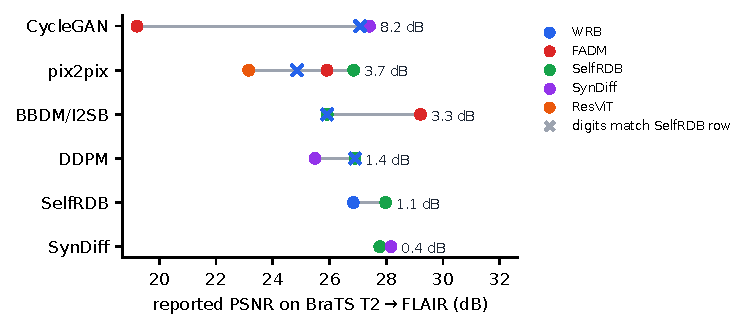
\includegraphics[width=\columnwidth]{figures/literature_protocols.pdf}
\caption{The same method as reported by different papers on BraTS T2$\to$FLAIR (crosses: WRB rows whose digits match a SelfRDB-paper row; BBDM and I$^2$SB share a row because WRB's ``BBDM'' equals SelfRDB's ``I$^2$SB''; SynDiff's own numbers are from unpaired training). The spread for one method with paired training (3.7~dB for pix2pix, 3.3~dB for BBDM/I$^2$SB; the 8.2~dB CycleGAN spread mixes paired and unpaired training) is as large as the gaps the papers report between methods, so the protocol, not the method, dominates cross-paper differences.}
\label{fig:lit}
\end{figure}

Table~\ref{tab:lit} and Fig.~\ref{fig:lit} make three points. First, the protocols differ in subject split (40 to 100 subjects, 10 to 20 test subjects), slice selection, resizing versus padding, normalization, masking and statistic unit, and several of these are not reported at all. Second, the same method moves by several decibels between papers (pix2pix from 23.15 to 26.85~dB; I$^2$SB from 25.92 to 29.21~dB), which is larger than most reported method-to-method gains. Third, several baseline rows of WRB's T2$\to$FLAIR table are digit-identical to rows of the SelfRDB paper, which used a different split (55 instead of 40 subjects), and in two cases the rows are attributed to differently named methods; we could not find a protocol under which both would be measured. We therefore do not rank our results against published numbers. Instead we retrain the reproducible baselines (pix2pix, SelfRDB) on our split, and we report a literature-protocol run only to calibrate how far the protocol moves PSNR.


\subsection{Baselines measured so far}
Table~\ref{tab:ours} lists what our single evaluation entry produces on \texttt{main\_val} today. The identity image metrics
do not depend on any training and are final. All lesion metrics use the smoke-test $\Seval$ (300 of the planned 20k steps)
and are only a pipeline check.

\begin{table*}[t]
\centering
\caption{Our protocol on main\_val (30 subjects), mean $\pm$ s.d.\ over subjects, single evaluation entry.
\prelim: preliminary $\Seval$ (300 of 20k steps), pipeline check only.}
\label{tab:ours}
\footnotesize
\setlength{\tabcolsep}{3pt}
\resizebox{\textwidth}{!}{%
\begin{tabular}{lcccc|cccccc}
\toprule
& \multicolumn{4}{c|}{Image quality (brain mask; LPIPS full slice)} & \multicolumn{6}{c}{Lesion level ($S_{\mathrm{eval}}$)} \\
Method & PSNR$\uparrow$ & SSIM$\uparrow$ & MAE$\downarrow$ & LPIPS$\downarrow$ & Dice$\uparrow$ & HD95$\downarrow$ & FP vol.\ ($10^3$)$\downarrow$ & Miss$\downarrow$ & SLR$\uparrow$ & EFA$\downarrow$ \\
\midrule
Identity (T2) & 11.90$\pm$2.41 & 0.250$\pm$0.171 & 0.218$\pm$0.085 & 0.165$\pm$0.025 & 0.39$\pm$0.27\prelim & 59.9\prelim & 77.8\prelim & 0.51\prelim & 0.32\prelim & 1.00\prelim \\
Real FLAIR (reference) & -- & -- & -- & -- & 0.77$\pm$0.17\prelim & 39.7\prelim & 15.6\prelim & 0.13\prelim & 0.34\prelim & 0.50\prelim \\
\midrule
UNet-$\ell_1$ & \pend & \pend & \pend & \pend & \pend & \pend & \pend & \pend & \pend & \pend \\
pix2pix & \pend & \pend & \pend & \pend & \pend & \pend & \pend & \pend & \pend & \pend \\
SelfRDB (retrained) & \pend & \pend & \pend & \pend & \pend & \pend & \pend & \pend & \pend & \pend \\
F0 (noise start) & \pend & \pend & \pend & \pend & \pend & \pend & \pend & \pend & \pend & \pend \\
F1 (ours, trunk) & \pend & \pend & \pend & \pend & \pend & \pend & \pend & \pend & \pend & \pend \\
F1 + lesion weight & \pend & \pend & \pend & \pend & \pend & \pend & \pend & \pend & \pend & \pend \\
F1 + seg.\ consistency & \pend & \pend & \pend & \pend & \pend & \pend & \pend & \pend & \pend & \pend \\
\bottomrule
\end{tabular}
}

\vspace{2pt}
{\footnotesize HD95 in voxels; FP vol.: voxels of $P$ farther than 5 voxels from the tumor; SLR: small-lesion recall (50 GT lesions $<$1000 voxels, pooled); EFA: false-alarm rate on 1161 tumor-free slices (pooled).}

\end{table*}

\begin{figure}[t]
\centering
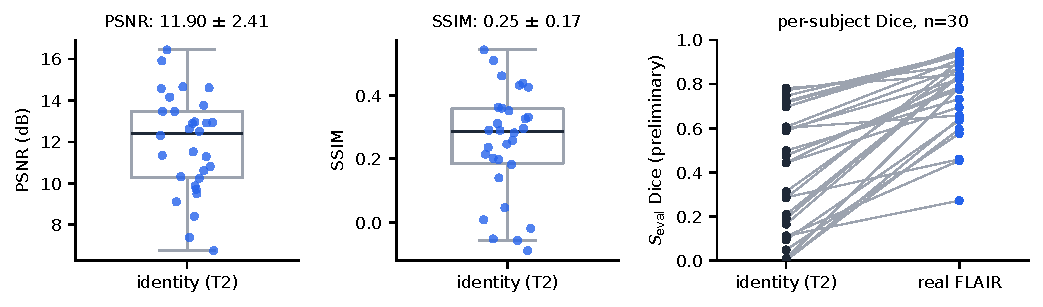
\includegraphics[width=\columnwidth]{figures/identity_baseline.pdf}
\caption{Per-subject baselines on main\_val. \emph{Left}: brain-mask PSNR and SSIM of the identity baseline (T2 used as
FLAIR). \emph{Right}: $\Seval$ Dice of the identity input and of real FLAIR, paired by subject (preliminary 300-step
$\Seval$). We hypothesize that identity reaches non-trivial Dice because $\Seval$ marks hyperintense T2 regions, which would also explain its large false-positive volume (Table~\ref{tab:ours}); lesion metrics must be read jointly.}
\label{fig:identity}
\end{figure}

Two observations already shape the analysis. First, under our brain-mask protocol the identity baseline scores 11.9\unskip~dB. This only
illustrates how strict brain-mask PSNR on per-volume normalized intensities is; it is not comparable with
Table~\ref{tab:lit}, and only the gap between a trained model and identity on the same protocol is interpretable. Second, identity T2 already obtains
a non-zero $\Seval$ Dice at the price of a very large false-positive volume and alarms on every tumor-free slice, plausibly because hyperintensity in T2 is not specific to tumor (CSF). With the preliminary $\Seval$ even real FLAIR raises alarms on half of the tumor-free slices, so this must be re-checked with the fully trained segmenter. A synthesis method that copies T2 contrast near the lesion would
therefore look acceptable in Dice alone; false-positive volume and empty-slice alarms expose it.

\subsection{Planned experiments}
Table~\ref{tab:plan} lists the planned comparisons. The trunk rule is fixed in its approved experiment card; the other rules are drafts that will be fixed, with margins and hyper-parameters, in their cards before running.

\begin{table}[t]
\centering
\caption{Planned experiments and draft decision rules (main\_val during development; main\_test once at the end).}
\label{tab:plan}
\footnotesize
\setlength{\tabcolsep}{3pt}
\begin{tabular}{>{\raggedright\arraybackslash}p{0.22\columnwidth}>{\raggedright\arraybackslash}p{0.33\columnwidth}>{\raggedright\arraybackslash}p{0.36\columnwidth}}
\toprule
Experiment & Question & Consequence \\
\midrule
Trunk F1 & PSNR gain over identity; Dice gap to real FLAIR & credible if $\geq$3~dB over identity and real-FLAIR Dice $\geq0.80$: lock trunk; else audit data/eval or switch to F0 \\
F0 vs.\ F1 & H1: does starting from T2 reduce FP volume at equal PSNR? & F1 kept if FP volume lower without PSNR loss \\
F1 + lesion weight ($\alpha{=}5$) & H2a: lower miss rate, small-lesion recall up? & adopted if miss rate drops and FP does not rise \\
F1 + seg.\ consistency & H2b: same, via $\Strain$ & adopted under the same rule; both combined only if both help \\
UNet-$\ell_1$, pix2pix, SelfRDB & where regression, GAN and a strong bridge sit on the same protocol & reference rows \\
Literature protocol & how much does the protocol move PSNR? & calibrates Table~\ref{tab:lit} \\
\bottomrule
\end{tabular}
\end{table}

\subsection{Status}
Preprocessing of the main protocol is complete and validated (counts and crop losses above). The full pipeline (training,
both segmenters, inference, evaluation, figures) has run end to end on real data in a smoke test. The trunk run (F1 for 50k
steps, then $\Seval$ and $\Strain$, about 11~h on one A100; the segmenters ran at about 0.05~s per step in the smoke test, roughly 20~min each) is queued. Qualitative results, including failure cases (lost
structure, artifacts, invented hyperintensities), will be selected from \texttt{main\_val} by a fixed rule: the subjects with
the largest false-positive volume and the largest miss rate.

% ---------------------------------------------------------------------------------------------
\section{Limitations (preliminary)}
The model is 2D with a 2.5D condition, so through-plane consistency is not enforced. Only one dataset (glioma) is used; white-matter
disease is not covered. Evaluator domain shift (Section~\ref{sec:eval}) can only be bounded, not removed, by the checks we plan. Brain-mask PSNR on per-volume normalized intensities is deliberately stricter than
whole-image PSNR and is not comparable to published numbers.

\appendix[Reviewer self-check (to resolve before submission)]
\begin{enumerate}
\item Is the lesion-level protocol a contribution beyond MPFlow-style segmentation Dice? (Needs: error types, identity and real-FLAIR references, evaluator
validity checks, per-subject tests.)
\item Does F1 beat SelfRDB, or only F0? The claim must match the result.
\item Is the $\Seval$ domain shift small enough that Dice differences reflect lesions? (Degraded-FLAIR check, error--Dice correlation.)
\item Is ``bridge flow matching'' distinguishable from BBDM/I$^2$SB? Only the controlled F0/F1 comparison is claimed.
\item Are improvements significant per subject on main\_test, with the test set used once?
\item Are failure cases shown, chosen by a rule rather than by hand?
\end{enumerate}

\bibliographystyle{IEEEtran}
\bibliography{refs}

\end{document}
